%!TEX root = practicum2.tex
We consider two different connectivities, namely four- and eight-connectivity, which are illustrated in \cref{fig:exp:connectivity}. In this section we discuss the influence of the 8-connectivity on the size of the cluster.

\Cref{fig:exp:connectivityResults} shows two clusters which have been grown using the same probabilities but different connectivities. \todo[inline]{Observaties.}

\begin{figure}
	\centering
	\begin{subfigure}{0.45\columnwidth}
		\centering
		\missingfigure{}
		\caption{4-connectivity}
		\label{fig:exp:connectivity:fourConnect}
	\end{subfigure}
	\begin{subfigure}{0.45\columnwidth}
		\centering
		\missingfigure{}
		\caption{8-connectivity}
		\label{fig:exp:connectivity:eightConnect}
	\end{subfigure}	
	\caption{The results of growing a cluster with the same grid of probabilites with \subref{fig:exp:connectivity:fourMask} four-connectivity and \subref{fig:exp:connectivity:eightMask} eight-connectivity.}
	\label{fig:exp:connectivityResults}
\end{figure}

\begin{figure}
	\centering
	\begin{subfigure}{0.45\columnwidth}
		\centering
		
\includegraphics[width=0.8\textwidth]{./img/exp_mask_four.jpg}
		\caption{4-connectivity}
		\label{fig:exp:connectivity:fourMask}
	\end{subfigure}
	\begin{subfigure}{0.45\columnwidth}
		\centering
		
\includegraphics[width=0.8\textwidth]{./img/exp_mask_eight.jpg}
		\caption{8-connectivity}
		\label{fig:exp:connectivity:eightMask}
	\end{subfigure}	
	\caption{Connectivity masks for \subref{fig:exp:connectivity:fourMask} four-connectivity and \subref{fig:exp:connectivity:eightMask} eight-connectivity. The red squares are considered neighbors of the blue center square.}
	\label{fig:exp:connectivity}
\end{figure}

% Influence of probability
The results of performing the same experiment as discussed in \cref{ss:exp:probability} with the eight-connectivity mask, are presented in \cref{fig:experiment:conn:mean_std_clusters} and \ref{fig:experiment:conn:p_inf_ratio}. We have changed the range of $p$ to $p = 0.2, 0,21, \dotsc, 0.99$, since using the range used for four-connectivity seemed too small.

It should be noted that for some values of $p$, especially larger values there are no mean cluster sizes, since no finite clusters were found. This indicates that one is much more likely to encounter a percolating cluster with eight-connectivity than with four-connectivity. \todo[inline]{Explain why this makes sense} \todo[inline]{Hoe zorgt dit ervoor dat de mean size van een cluster kleiner is?}

This is confirmed by \cref{fig:experiment:conn:p_inf_ratio}, where we find that only for very low values of $p$ $P_\infty$ is zero, and that $P_\infty$ quickly approaches 1. 

These findings suggest that $p_c$ is much lower when eight-connectivity is used. Based on this, admittedly small experiment, one would guess $p_c$ to be approximately $0.2$ when eight-connectivity is used. More research is needed to find the actual value of $p_c$ when eight-connectivity is used.\\

\begin{figure*}
	\centering
	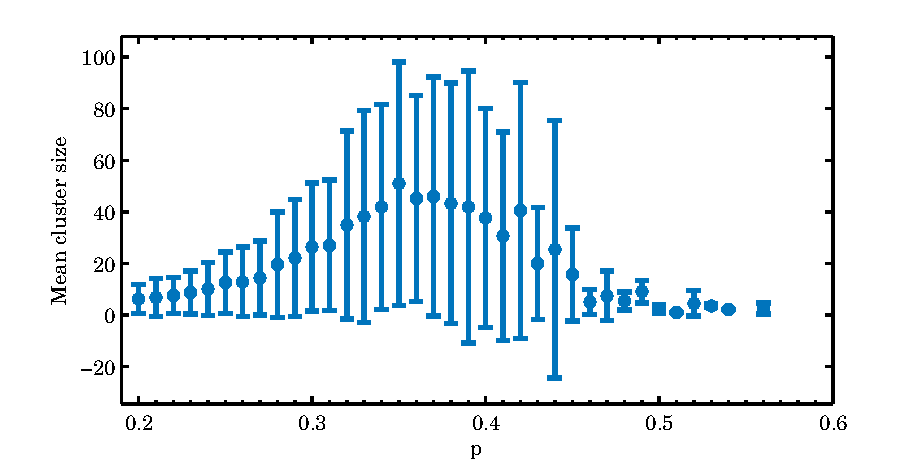
\includegraphics[width=\textwidth]{./img/assignment_d_mean_std_p.pdf}
	\caption{Mean cluster sizes, represented as points, and standard deviations, indicated by the vertical error bars, as a function of $p = 0.2, 0,21, \dotsc, 0.99$ when eight-connectivity is used. The mean and standard deviation were calculated over $200$ runs on a $41 \times 41$ grid.}
	\label{fig:experiment:conn:mean_std_clusters}
\end{figure*}

\begin{figure}
	\centering
	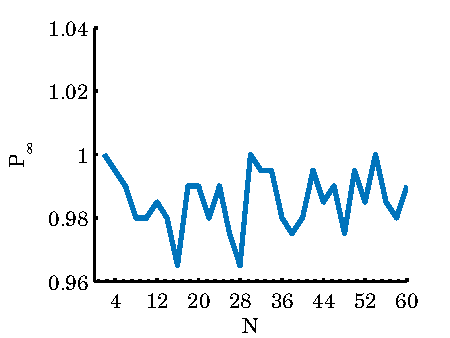
\includegraphics[width=\columnwidth]{./img/assignment_d_p_infinite_ratio_p.pdf}
	\caption{Ratio of percolating clusters, $P_\infty$, as a function of $p = 0.2, 0,21, \dotsc, 0.99$ when eight-connectivity is used. Ratios are calculated over $r_{max} = 200$ runs on a $41 \times 41$ grid.}
	\label{fig:experiment:conn:p_inf_ratio}
\end{figure}

\todo{Influence of size}
% To determine the influence of the connectivity on the size we have performed the same experiment as used for the four-connectivity. \todo[inline]{Resultaten}

\todo{Influence on fractal dimension}
% We have determined the fractal dimension of the cluster generated using four connectivity for $N = 80$ and $p =0.7$. We have found that \todo[inline]{Resulaten}

